\documentclass[border=2mm]{standalone}
\usepackage{tikz}
\usetikzlibrary{positioning}

\definecolor{mybluei}{RGB}{124,156,205}
\definecolor{myblueii}{RGB}{73,121,193}
\definecolor{mygreen}{RGB}{202,217,126}

\pgfdeclarelayer{background}
\pgfsetlayers{background,main}

\begin{document}

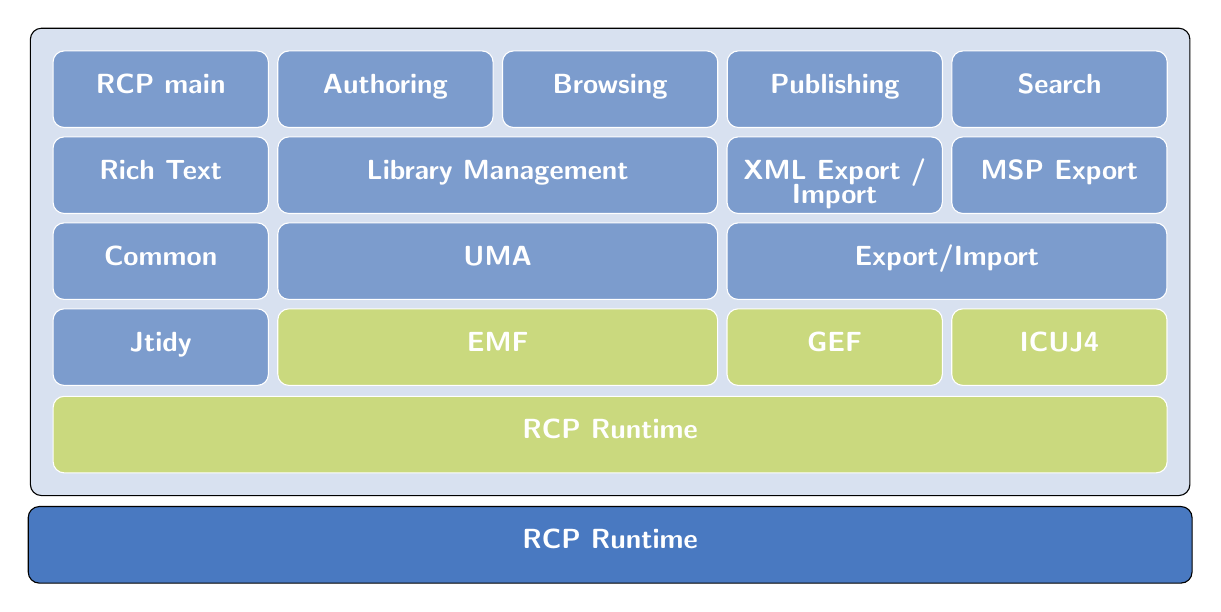
\begin{tikzpicture}[node distance=3pt,
blueb/.style={
  draw=white,
  fill=mybluei,
  rounded corners,
  text width=2.5cm,
  font={\sffamily\bfseries\color{white}},
  align=center,
  text height=12pt,
  text depth=9pt},
greenb/.style={blueb,fill=mygreen},
]
\node[blueb] (RCP) {RCP main};
\node[blueb,right=of RCP] (Aut) {Authoring};
\node[blueb,right=of Aut] (Bro) {Browsing};
\node[blueb,right=of Bro] (Pub) {Publishing};
\node[blueb,right=of Pub] (Sea) {Search};
\node[blueb,below=of RCP] (RTe) {Rich Text};
\node[blueb,right=of RTe,text width=5cm+10pt] (LMa) {Library Management};
\node[blueb,right=of LMa] (XML) {XML Export /\\[-0.7ex] Import};
\node[blueb,right=of XML] (MSP) {MSP Export};
\node[blueb,below=of RTe] (Com) {Common};
\node[blueb,right=of Com,text width=5cm+10pt] (UMA) {UMA};
\node[blueb,right=of UMA,text width=5cm+10pt] (EI) {Export/Import};
\node[blueb,below=of Com] (Jti) {Jtidy};
\node[greenb,right=of Jti,text width=5cm+10pt] (EMF) {EMF};
\node[greenb,right=of EMF] (GEF) {GEF};
\node[greenb,right=of GEF] (ICU) {ICUJ4};
\node[greenb,below=3.4cm of Bro,text width=13cm+26pt] (RCP) {RCP Runtime};
\begin{pgfonlayer}{background}
\draw[blueb,draw=black,fill=mybluei!30] 
  ([xshift=-8pt,yshift=8pt]current bounding box.north west) rectangle 
  ([xshift=8pt,yshift=-8pt]current bounding box.south east);
\end{pgfonlayer}
\node[blueb,draw=black,fill=myblueii,below=4.8cm of Bro,text width=13cm+44pt] (RCP) {RCP Runtime};

\end{tikzpicture}

\end{document}